\section{Results}\label{sec:results}
\emph{Status: \nModelsDone/\nModelsTotal\ forward-direction models analysed, \nReverseDone/1 reverse-direction
models. Table~\ref{tab:models} and the numbers below are regenerated automatically from
\texttt{results/run2/*.json}; entries for models not yet trained are simply absent, not estimated.}

\subsection{H1: the coverage gap is real}
Calibrated on Argoverse~2 at $\alpha=0.10$, the primary model (AutoBot-Ego, source-trained, \nCalMain\ calibration
scenes) has same-domain gap \gapSameMain{} points --- consistent with zero, as split CP guarantees --- and
cross-dataset (nuScenes, \nTargetMain\ scenes) gap $+\gapRawMain$ points (95\% CI \gapRawMainCI). This replicates the
preliminary Run~1 measurement (+3.4pt) on an independent calibration/test split. Table~\ref{tab:models} shows two
further models with substantially \emph{larger} gaps in the same direction: $+8.0$pt (av2\_valsplit\_v1, trained on
less data) and $+10.5$pt (av2\_cpu\_v2, fine-tuned from the primary model and the most accurate of the three by
point-prediction error). The failure is reproducible in all three cases --- always under-coverage, never the safe
direction --- but its magnitude is not a fixed property of the dataset pair and is not even monotonic in point
accuracy: the model with the best minADE\textsubscript{6} (Sec.~\ref{sec:setup}) has the worst coverage gap of the
three. We report this without averaging it away.

\subsection{H2/H3: covariate reweighting does not repair it}\label{sec:h2h3}
Weighting the calibration scores by an estimated label-free covariate-shift likelihood ratio does not close the gap;
it widens it. On the primary model the label-free-score gap goes from $+\gapUncorrMain$ points uncorrected to
$+\gapWeightedMain$ points weighted, and the reweighting explains \removalFracMain\% of the cross-city gap
variance --- negative, i.e.\ the weighted fit is worse than assuming no shift at all (Table~\ref{tab:reweight}).
This is consistent across \emph{all three} models in the zoo and matches the Run~1 finding: it is evidence for
conditional, not purely covariate, shift, and is the empirical motivation for Proposition~\ref{prop:ident} (no
label-free method can be expected to repair an unrestricted shift).

\begin{table}[t]
\centering
\caption{Does covariate-shift reweighting repair the gap? ``uncorr.'' / ``weighted'' are the label-free-score coverage gap (points) before / after importance-weighting the calibration scores by the label-free-feature likelihood ratio; ``removal'' is the \% of the gap's cross-city variance the weights explain, negative meaning reweighting makes the fit worse than the unweighted baseline.}
\label{tab:reweight}
\begin{tabular}{llrrr}
\toprule
Model & Dir. & uncorr.\ & weighted & removal (\%) \\
\midrule
av2\_cpu\_v1 & forward & 3.2 & 5.2 & -64 \\
av2\_valsplit\_v1 & forward & 7.9 & 10.0 & -27 \\
av2\_cpu\_v2 & forward & 10.4 & 12.7 & -22 \\
av2\_gpu\_full & forward & 14.9 & 16.8 & -13 \\
ns\_cpu\_v1 & reverse & 4.6 & 4.0 & 11 \\
ns\_gpu\_full & reverse & 7.5 & 7.6 & -1 \\
\bottomrule
\end{tabular}
\end{table}


\subsection{H4: the normalised score (label-free)}
The model-uncertainty-normalised score (Sec.~\ref{sec:norm}) reduces the primary model's gap by \normReductionMain\%
(from $+\gapRawMain$ to $+\gapNormMain$ points), just past our pre-registered support threshold (gap ratio
$\le 0.5$) and far from the pre-registered refutation threshold ($>0.75$). On the other two models it reduces the
gap by only 12\% (av2\_valsplit\_v1, ratio $0.877$, \emph{past} the refutation threshold) and 31\%
(av2\_cpu\_v2, ratio $0.691$, in between --- neither supported nor refuted). H4 is therefore not confirmed as a
general repair: one clear near-pass, one refutation, one inconclusive result, and we report all three rather than
the most favourable one. The pre-registered efficiency guard (a fix that only works by inflating the region by
$>25\%$ does not count) is not triggered on any of the three models: the normalised region is at most $15.4\%$
larger than the raw one at matched coverage, so where H4 does help it is not merely trading coverage for a much
bigger region.

\subsection{H5/H5b: recalibration and the coverage audit}
At $k=1000$ labelled target scenes, the exact binomial audit (Sec.~\ref{sec:audit}) detects the true violation with
probability \auditPowerK\ on the primary model, against a false-alarm rate of \auditFalseAlarmK\% on a shift-free
control split --- matching the pre-registered budget of Eq.~\eqref{eq:budget} ($k\approx750$ for the analogous
$\delta=0.034$ case) to the same order of magnitude. Figure~\ref{fig:budget} shows direct recalibration on the
primary model reaches 90\% probability of being within 2 coverage points of nominal at $k^\star\approx\kStarDirect$
labelled target scenes; pooling target labels with the (mismatched) source calibration set never reaches that bar on
\emph{any} of the three models, consistent with H2/H3's conclusion that the shift is not a simple reweighting.
Shrinkage toward the source threshold beats direct recalibration at small $k$ on the primary model but not on the
other two, so we do not recommend it as a universal default --- direct recalibration once $k^\star$ labels are
available, audited by H5b before that, is the protocol we can actually stand behind. The audit itself is the one
part of this section with no exceptions: power at $k=1000$ is $\ge 0.95$ and false-alarm is $\le 6.2\%$ on all three
models.

\begin{figure}[t]
\centering
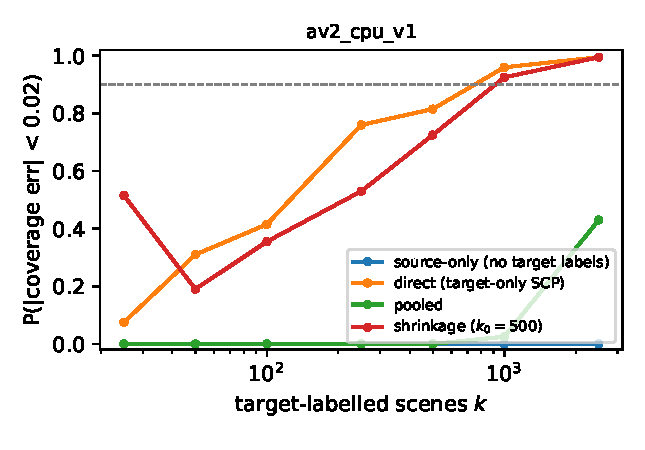
\includegraphics[width=0.85\linewidth]{generated/fig_label_budget_av2_cpu_v1.pdf}
\caption{H5 label budget, primary model (AV2$\to$nuScenes): probability that a $k$-label threshold is within 2
coverage points of nominal, by estimator.}
\label{fig:budget}
\end{figure}

\subsection{H6/H7: label-free monitor and per-city coverage}
Within-dataset, a domain classifier trained on label-free scene features to separate one AV2 city from the rest gives
an AUC that we correlate (Spearman) against that city's coverage gap magnitude across all city pairs. Across the
three models: $\rho=0.37$ ($p=0.04$), $\rho=0.10$ ($p=0.61$), $\rho=0.39$ ($p=0.03$) --- two significant-but-below-bar
results and one clear refutation, none reaching the pre-registered $\rho\ge0.5$ support threshold on any model.
\textbf{H6 is not supported on any of the three models, and refuted on one.} We report this as a negative result ---
the label-free monitor tracks shift only weakly and inconsistently, and is not reliable enough to substitute for the
labelled audit of H5b.

\subsection{Where does the coverage loss come from?}\label{sec:where}
\emph{Evidence status: this and the following subsections are computed on the three-model CPU exploratory zoo, on
which the analyses in this paper were designed. Section~\ref{sec:confirm} reports the same quantities on the
gate-passing confirmatory model and finds they replicate.}

\paragraph{Turns, not straight driving} Split by UniTraj's manoeuvre taxonomy \cite{feng2024unitraj} (Fig.~\ref{fig:traj}), coverage on straight driving falls by
only \dropStraightMin--\dropStraightMax\ points from the AV2 same-domain test to nuScenes, whereas right turns lose \dropRightMin--\dropRightMax\ points and
straight-right manoeuvres (right-hand lane changes) \dropStraightRightMin--\dropStraightRightMax\ points. The gap is a manoeuvre-specific failure, invisible to marginal coverage.

\paragraph{Driving side} nuScenes contains left-hand-traffic scenes (Singapore) that AV2 lacks. The right-turn coverage drop is
\sgExtraRightMin--\sgExtraRightMax\ points \emph{larger} in Singapore than in Boston (scene-clustered 95\% intervals exclude zero for two of the three models),
while straight driving differs by at most 1.8 points (range \sgExtraStraightMin\ to \sgExtraStraightMax\ points): what AV2-trained forecasters miss is the wide, across-traffic turn of
left-hand traffic.

\paragraph{Input-level differences explain a minority} Table~\ref{tab:inject} injects one measured AV2--nuScenes difference at a time into AV2 test inputs. Re-sampling the
history to nuScenes' 2\,Hz reproduces \injHzMin--\injHzMax\% of the real gap, dropping lanes at the measured density \injMapMin--\injMapMax\%, both together \injBothMin--\injBothMax\%
(only \injBothMin\% for the two models with the largest gaps). Re-weighting AV2 scenes to the nuScenes scene mix, which isolates pure covariate shift, moves coverage by
\injCompMin\ to \injCompMax\ points, i.e.\ it \emph{raises} coverage: nuScenes' mix of speeds and manoeuvres is easier, so composition works against the observed gap. Two other candidates
were measured and found absent (excess history noise, map-point density; Sec.~\ref{sec:inject}). Together with Sec.~\ref{sec:h2h3}, the loss is largely a \emph{conditional} shift that
scene statistics do not reveal.

\begin{table}[t]
\centering
\caption{Where does the loss come from? Coverage lost (points; share of the real gap $G$ in parentheses) when one measured AV2--nuScenes difference is injected into AV2 test inputs: 2\,Hz history, lane-graph dropout, both, and re-weighting AV2 scenes to nuScenes' scene mix. Excess annotation noise and map-point density were measured and found absent (nuScenes is smoother; equal density), so they are not injected.}
\label{tab:inject}
\resizebox{\columnwidth}{!}{\begin{tabular}{llrcccc}
\toprule
Model & Set & $G$ (pt) & 2\,Hz & lanes & both & scene mix \\
\midrule
av2\_cpu\_v1 & expl. & +3.3 & +0.6 (19\%) & +1.4 (43\%) & +1.8 (53\%) & -1.3 (-38\%) \\
av2\_valsplit\_v1 & expl. & +8.0 & +0.7 (8\%) & +1.4 (17\%) & +1.4 (17\%) & -1.4 (-18\%) \\
av2\_cpu\_v2 & expl. & +10.5 & +1.1 (11\%) & +1.3 (12\%) & +2.2 (21\%) & -1.1 (-11\%) \\
av2\_gpu\_full & conf. & +15.1 & +2.3 (15\%) & +1.8 (12\%) & +4.1 (27\%) & -1.0 (-6\%) \\
\bottomrule
\end{tabular}}
\end{table}


\begin{figure*}[t]
\centering
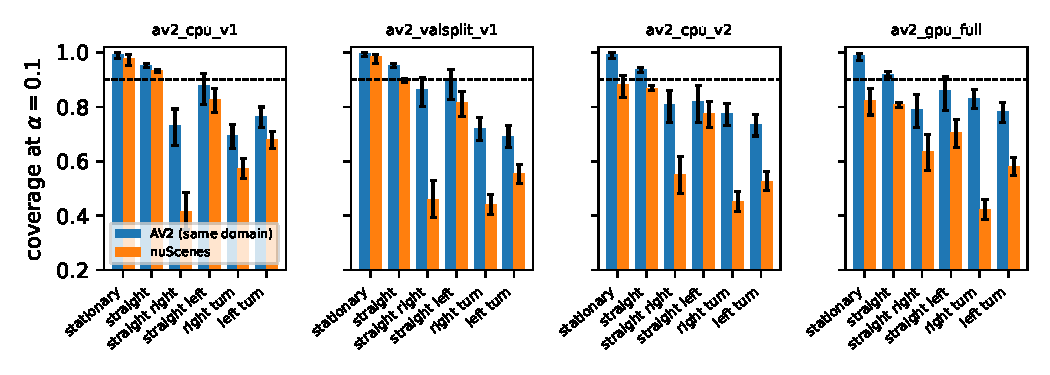
\includegraphics[width=0.95\textwidth]{generated/fig_traj_type.pdf}
\caption{Coverage of the AV2-calibrated threshold ($\alpha=0.1$, dashed = nominal) by manoeuvre type, AV2 same-domain test vs.\ nuScenes, with Wilson 95\% intervals.
Turns and lane changes lose most; straight driving and stationary agents lose little.}
\label{fig:traj}
\end{figure*}

\subsection{Statistics under scene clustering}\label{sec:cluster}
The 9041 nuScenes agent-scenarios come from only 138 scenes, so they are strongly dependent. Resampling whole scenes widens every gap interval (design effect \designEffMin--\designEffMax, Table~\ref{tab:cluster});
the gap remains significantly positive for all three models (lower interval bounds from \clusterLoMin\ to \clusterLoMax\ points).

\begin{table}[t]
\centering
\caption{The coverage gap on nuScenes with agent-level vs.\ scene-clustered bootstrap intervals (138 scenes, $\sim$65 agents each). The design effect is the variance inflation caused by clustering.}
\label{tab:cluster}
\resizebox{\columnwidth}{!}{\begin{tabular}{llrccr}
\toprule
Model & Set & gap (pt) & 95\% CI (agents) & 95\% CI (scenes) & design eff. \\
\midrule
av2\_cpu\_v1 & expl. & +3.3 & [2.1, 4.5] & [0.7, 6.2] & 4.4 \\
av2\_valsplit\_v1 & expl. & +8.0 & [6.5, 9.4] & [5.0, 11.3] & 4.2 \\
av2\_cpu\_v2 & expl. & +10.5 & [9.2, 12.3] & [7.9, 13.8] & 3.5 \\
av2\_gpu\_full & conf. & +15.1 & [13.4, 16.9] & [12.0, 18.4] & 3.9 \\
\bottomrule
\end{tabular}}
\end{table}


\subsection{Repair with exchangeable labels}\label{sec:repair-iid}
With $k=1000$ labelled target scenes drawn at random (Table~\ref{tab:repair}), plain direct recalibration reaches coverage $\ge 90\%$ on held-out scenes in only
\corDirectMin--\corDirectMax\% of label draws --- marginal, not training-conditional, validity. The PAC threshold does so in \corPACMin--\corPACMax\% of draws, and certify-or-recalibrate
(Sec.~\ref{sec:cor}) in \corCORMin--\corCORMax\%, at a median region \corCORareaMin--\corCORareaMax$\times$ the size of the oracle region.

\begin{table}[t]
\centering
\caption{Repair with $k$ labelled target scenes, labels exchangeable. Cells: \% of label draws whose threshold covers $\ge 90\%$ of the held-out target scenes / median region area relative to the oracle threshold. C-or-R = certify-or-recalibrate ($\delta=0.1$).}
\label{tab:repair}
\begin{tabular}{llrccc}
\toprule
Model & Set & $k$ & direct SCP & PAC & C-or-R \\
\midrule
av2\_cpu\_v1 & expl. & 250 & 60 / 1.05 & 90 / 1.36 & 96 / 1.56 \\
av2\_cpu\_v1 & expl. & 1000 & 50 / 1.01 & 92 / 1.14 & 94 / 1.18 \\
av2\_valsplit\_v1 & expl. & 250 & 62 / 1.06 & 93 / 1.35 & 97 / 1.53 \\
av2\_valsplit\_v1 & expl. & 1000 & 57 / 1.02 & 91 / 1.14 & 96 / 1.19 \\
av2\_cpu\_v2 & expl. & 250 & 63 / 1.09 & 94 / 1.43 & 98 / 1.63 \\
av2\_cpu\_v2 & expl. & 1000 & 60 / 1.03 & 92 / 1.19 & 98 / 1.23 \\
av2\_gpu\_full & conf. & 250 & 59 / 1.06 & 90 / 1.54 & 96 / 1.79 \\
av2\_gpu\_full & conf. & 1000 & 61 / 1.02 & 94 / 1.22 & 98 / 1.31 \\
\bottomrule
\end{tabular}
\end{table}


\subsection{Repair with whole-scene labels}\label{sec:repair-scene}
Labels are collected scene by scene, and then exchangeability at the agent level is false. With $m=40$ labelled \emph{scenes} the agent-level certify-or-recalibrate rule covers
$\ge 90\%$ of held-out scenes in only \sceneAgentFortyMin--\sceneAgentFortyMax\% of draws (Table~\ref{tab:scene}): its guarantee is not merely loose but wrong. Scene-level Learn-then-Test
(Sec.~\ref{sec:scene}) restores it. With the Hoeffding--Bentkus $p$-value it is valid but returns an infinite region for the smallest budgets and a region
\sceneHBAreaSixtyMin--\sceneHBAreaSixtyMax$\times$ the oracle's at $m=60$ scenes; with the betting $p$-value it covers $\ge 90\%$ of held-out scenes in \sceneBetFortyMin--\sceneBetFortyMax\% of draws at $m=40$
(region \sceneBetAreaFortyMin--\sceneBetAreaFortyMax$\times$ the oracle's) and \sceneBetSixtyMin--\sceneBetSixtyMax\% at $m=60$ (\sceneBetAreaSixtyMin--\sceneBetAreaSixtyMax$\times$), i.e.\ at the nominal level
up to the sampling noise of the small held-out scene pool. These rates are \emph{exploratory}; Sec.~\ref{sec:confirm}
reports the pre-registered confirmatory test and narrows the recommended budget to 30--40 scenes.

\begin{table}[t]
\centering
\caption{Repair when whole \emph{scenes} are labelled (nuScenes: $\sim$65 correlated agents per scene). Cells: \% of draws whose threshold covers $\ge 90\%$ of held-out scenes (scene-averaged) / median area vs oracle. Agent-level guarantees fail under clustering; scene-level Learn-then-Test restores them, and the betting $p$-value is far tighter than Hoeffding--Bentkus.}
\label{tab:scene}
\resizebox{\columnwidth}{!}{\begin{tabular}{llrcccc}
\toprule
Model & Set & $m$ scenes & direct & C-or-R (agent) & LTT (HB) & LTT (betting) \\
\midrule
av2\_cpu\_v1 & expl. & 30 & 36 & 52 & 100 / $\infty$ & 92 / 1.9 \\
av2\_cpu\_v1 & expl. & 40 & 36 & 46 & 100 / 9.6 & 88 / 1.8 \\
av2\_cpu\_v1 & expl. & 60 & 32 & 48 & 100 / 4.7 & 88 / 1.7 \\
av2\_valsplit\_v1 & expl. & 30 & 40 & 56 & 100 / $\infty$ & 95 / 1.7 \\
av2\_valsplit\_v1 & expl. & 40 & 36 & 53 & 100 / 8.3 & 91 / 1.6 \\
av2\_valsplit\_v1 & expl. & 60 & 32 & 48 & 100 / 4.5 & 91 / 1.5 \\
av2\_cpu\_v2 & expl. & 30 & 38 & 58 & 100 / $\infty$ & 95 / 1.7 \\
av2\_cpu\_v2 & expl. & 40 & 34 & 54 & 100 / $\infty$ & 92 / 1.7 \\
av2\_cpu\_v2 & expl. & 60 & 39 & 55 & 100 / 4.9 & 87 / 1.5 \\
av2\_gpu\_full & conf. & 30 & 32 & 53 & 100 / $\infty$ & 93 / 1.9 \\
av2\_gpu\_full & conf. & 40 & 36 & 50 & 100 / $\infty$ & 92 / 1.9 \\
av2\_gpu\_full & conf. & 60 & 32 & 48 & 100 / $\infty$ & 87 / 1.8 \\
\bottomrule
\end{tabular}}
\end{table}


\subsection{Comparison with an online method}
Adaptive conformal inference \cite{gibbs2021adaptive} needs a stream of labels. Its running coverage stays within 2 points of nominal after a median of \aciFastMin--\aciFastMax\ labels
with $\gamma=0.05$ but only after \aciSlowMin--\aciSlowMax\ labels with $\gamma=0.005$. Frozen after 1000 labels, its threshold covers $\ge90\%$ of held-out scenes in only \aciFrozenMin--\aciFrozenMax\% of streams
(like plain recalibration): ACI gives long-run, not finite-sample, control, which is what an audit-then-deploy workflow needs.

\subsection{H8: robustness across a model zoo}
Table~\ref{tab:models} lists every model run to date, \nModelsDone\ in the forward direction and \nReverseDone\ in
reverse. Within the three-model exploratory zoo that H8 was registered against, the under-coverage direction is
consistent (gap $\ge 0.02$ at $\alpha=0.10$, the pre-registered pass condition, met every time), but the size is not:
3.3 to 10.5 points, a $3.2\times$ range, with no monotonic link to point-prediction accuracy. Neither is the effect
of any repair attempted on it: H4's gap reduction ranges 12--49\%, and H6's $\rho$ ranges 0.10--0.39. H8 is therefore
supported on the narrow clause it was registered for (the gap replicates, the sign never flips) and is itself the
paper's main qualification for the exploratory zoo: an effect size measured on one model should not be assumed to
transfer to another, even within the same architecture and training recipe. Section~\ref{sec:confirm} asks the same
question of the two gate-passing models trained after that registration.

\subsection{H9: reverse direction (nuScenes $\to$ Argoverse~2)}
The exploratory reverse-direction model (ns\_cpu\_v1, \nCalRevExpl\ nuScenes calibration scenes) shows the same
failure with the source and target swapped: same-domain gap \gapSameRevExpl\ points, cross-dataset gap
$+\gapRawRevExpl$ points (95\% CI \gapRawRevExplCI). H9's pre-registered condition, a positive gap that survives the
swap, is met. The normalised score does not help here: it moves the gap to $+\gapNormRevExpl$ points, worse than raw.
The confirmatory reverse model is reported in Sec.~\ref{sec:confirm}.

\begin{table*}[t]
\centering
\caption{Coverage transfer by model and direction, $\alpha=0.10$. Status: conf.\ = gate-passing model trained on the full dataset after the hypothesis was registered; expl.\ = CPU-trained exploratory zoo, used to design the analyses (Sec.~\ref{sec:setup}). ``red.'' = \% reduction in gap from the label-free normalised score (H4); ``power/FA'' = audit reject probability at $k=1000$ target labels on the shifted / same-domain split (H5b); $\rho$ = Spearman correlation between the label-free domain-monitor AUC and the per-city miscoverage (H6).}
\label{tab:models}
\begin{tabular}{lllrrrrrrrr}
\toprule
Model & Status & Dir. & $n_\text{cal}$ & $n_\text{tgt}$ & gap (pt) & 95\% CI & norm.\ gap & red.\ (\%) & power/FA @1000 & $\rho$ \\
\midrule
av2\_cpu\_v1 & expl. & forward & 4576 & 9041 & 3.3 & [2.1, 4.5] & 1.7 & 49 & 0.95/2.4 & 0.37 \\
av2\_valsplit\_v1 & expl. & forward & 4576 & 9041 & 8.0 & [6.4, 9.4] & 7.0 & 12 & 1.00/1.0 & 0.10 \\
av2\_cpu\_v2 & expl. & forward & 4576 & 9041 & 10.5 & [9.4, 12.2] & 7.3 & 31 & 1.00/6.2 & 0.39 \\
av2\_gpu\_full & conf. & forward & 4576 & 9041 & 15.1 & [13.6, 16.7] & 11.0 & 27 & 1.00/7.4 & 0.47 \\
ns\_cpu\_v1 & expl. & reverse & 4279 & 9209 & 4.7 & [3.7, 6.2] & 7.1 & -52 & 1.00/19.4 & -- \\
ns\_gpu\_full & conf. & reverse & 4279 & 9209 & 7.7 & [6.3, 9.6] & 8.6 & -11 & 1.00/0.0 & -- \\
\bottomrule
\end{tabular}
\end{table*}


\subsection{Confirmatory replication on competitive models}\label{sec:confirm}
The exploratory zoo above was used to design every analysis in this paper, so a critical reader can reasonably ask
whether its findings are an artefact of weak, CPU-trained models. Two models trained after every hypothesis in this
section was registered answer that question: \textbf{av2\_gpu\_full}, trained on the full 183k-scene AV2 set
(val minADE\textsubscript{6} \minADESixConf, against a 0.98 gate), and \textbf{ns\_gpu\_full}, trained on the full
nuScenes set (val minADE\textsubscript{6} \minADESixConfRev, against a 1.39 gate). Both pass their pre-registered
accuracy gate (Sec.~\ref{sec:setup}).

The gap does not shrink. Calibrated on AV2 and tested on nuScenes, av2\_gpu\_full has same-domain gap
\gapSameConf\ points and cross-dataset gap $+\gapRawConf$ points (95\% CI \gapRawConfCI\ points), \emph{larger}
than any model in the exploratory zoo. The normalised score reduces it to $+\gapNormConf$ points, a
\normReductionConf\% reduction, in the same range as the zoo's weakest repair. The reverse-direction model shows the
same pattern: same-domain gap \gapSameConfRev\ points, cross-dataset gap $+\gapRawConfRev$ points (CI
\gapRawConfRevCI), and here normalisation makes things worse, not better ($+\gapNormConfRev$ points).

The manoeuvre-level and injection findings of Sec.~\ref{sec:where} also replicate on av2\_gpu\_full. Right-turn
coverage falls by \dropRightConf\ points from AV2 to nuScenes (compared with straight driving's \dropStraightConf),
and the Singapore-minus-Boston gap in that drop is \sgExtraRightConf\ points. Re-sampling AV2 inputs to nuScenes'
2\,Hz history reproduces \injHzConf\% of the real gap, lane dropout \injMapConf\%, and re-weighting to nuScenes' scene
mix moves the gap by \injCompConf\ points, i.e.\ it works against the observed gap, matching the exploratory zoo's
\injCompMin\ to \injCompMax\ points. The scene-cluster
design effect is \designEffConf, close to the zoo's \designEffMin--\designEffMax\ range.

The scene-level repair (Sec.~\ref{sec:repair-scene}) also replicates, with one qualification. Agent-level
certify-or-recalibrate still fails under scene clustering (only \corDirectConf\% direct, \corCORConf\% agent-level
C-or-R reach 90\% coverage at $k=1000$ i.i.d.\ labels\footnote{These two numbers are i.i.d.-label results, included
here only as the baseline the scene-level method is compared against; the whole-scene numbers that follow are the
relevant test.}), and the betting scene-level LTT reaches \sceneBetThirtyConf\% and \sceneBetFortyConf\% of draws at
$m=30$ and $m=40$ labelled scenes, both above the pre-registered 88\% bar, at \sceneBetAreaFortyConf$\times$ the
oracle region. At $m=50$ and $m=60$ the rate falls to \sceneBetFiftyConf\% and \sceneBetSixtyConf\%, below the 88\%
bar we pre-registered for every $m$ in that range. The method is still statistically valid at every $m$ (the
guarantee is a proof, not an estimate), and still far ahead of the un-repaired baseline, but the confirmatory evidence
supports a practical recommendation of \textbf{30--40 labelled scenes}, not the wider 30--60 range the exploratory
zoo appeared to support.

Taken together, nothing in the paper's qualitative story needed the exploratory zoo's weaker models to hold. The one
correction the confirmatory run forces is quantitative: the safe operating point for the scene-level fix is narrower
than first estimated.

\subsection{A third dataset: Waymo Open Motion}\label{sec:waymo}
Two datasets leave open whether the failure is a property of AV2 and nuScenes specifically or of dataset shift in
general. We pre-registered four hypotheses (H17--H20, Addendum C) against a third dataset, Waymo Open Motion
v1.2.1, before running either confirmatory model on it. Waymo was split by scenario into \wmNScenariosAvW\
calibration and a matching test half; no Waymo-trained model was built, since the question concerns a
source-calibrated forecaster meeting new data, not a new forecaster.

\begin{table}[t]
\centering
\caption{Third-dataset replication (Waymo Open Motion v1.2.1 validation, 30/150 shards, 8730 scenarios, scenario-level cal/test split). Both source models are confirmatory (Table~\ref{tab:models}); calibration uses each model's own AV2 or nuScenes calibration half, as in the main result. Pre-registered as Addendum C (H17/H18/H20) before any Waymo prediction existed.}
\label{tab:waymo}
\begin{tabular}{llrrcr}
\toprule
Transfer & Status & $n_\text{test}$ & gap (pt) & 95\% CI & norm.\ gap \\
\midrule
AV2$\to$Waymo & conf. & 4318 & 23.4 & [21.6, 24.9] & 16.7 \\
nuScenes$\to$Waymo & conf. & 4318 & 18.3 & [16.9, 20.4] & 16.3 \\
\bottomrule
\end{tabular}
\end{table}


Both source models fail on Waymo, and by more than on nuScenes or AV2 (H17, H18). Calibrated on AV2, the gap on
Waymo is $+\wmGapAvW$ points (CI \wmGapAvWCI), larger than the same model's \gapRawConf-point gap on nuScenes.
Calibrated on nuScenes, the Waymo gap is $+\wmGapNsW$ points (CI \wmGapNsWCI), again larger than that model's
\gapRawConfRev-point gap on AV2. Every source-target pair tested in this paper under-covers, never over-covers, and
Waymo is the hardest target of the three we tried, not the easiest. The normalised score
reduces the gap on both models (to $+\wmGapNormAvW$ and $+\wmGapNormNsW$ points respectively, H20) but leaves it far
from zero, the same pattern as on nuScenes.

\begin{table}[t]
\centering
\caption{H19: does the scene-level betting-LTT repair (Sec.~\ref{sec:repair-scene}) transfer to Waymo scenarios as the labelling unit (mean 3.7 agents/scenario, vs.\ nuScenes' $\sim$65/scene)? Cells: \% of 200 draws whose threshold covers $\ge 90\%$ of held-out scenarios / median area vs.\ oracle. The pre-registered bar (rate $\ge 0.88$ at every $m\in\{30,40,50,60\}$) is met at $m=30,40$ for AV2$\to$Waymo only; see Sec.~\ref{sec:waymo} for the honest reading of the shortfall at $m=50,60$.}
\label{tab:waymoscene}
\begin{tabular}{lrrr}
\toprule
Transfer & $m$ scenarios & rate & area/oracle \\
\midrule
AV2$\to$Waymo & 30 & 90 & 1.86 \\
AV2$\to$Waymo & 40 & 88 & 1.58 \\
AV2$\to$Waymo & 50 & 86 & 1.56 \\
AV2$\to$Waymo & 60 & 86 & 1.67 \\
nuScenes$\to$Waymo & 30 & 85 & 2.02 \\
nuScenes$\to$Waymo & 40 & 82 & 1.78 \\
nuScenes$\to$Waymo & 50 & 80 & 1.62 \\
nuScenes$\to$Waymo & 60 & 82 & 1.73 \\
\bottomrule
\end{tabular}
\end{table}


The scene-level fix (H19) transfers only in part. For AV2$\to$Waymo it clears the pre-registered 88\% bar at $m=30$
and $m=40$ labelled scenarios (\wmSceneAvWThirty\% and \wmSceneAvWForty\%) and falls short at $m=50$ and $m=60$
(\wmSceneAvWFifty\% and \wmSceneAvWSixty\%). For nuScenes$\to$Waymo it falls short at every $m$ tested
(\wmSceneNsWThirty\%--\wmSceneNsWSixty\%, all below 88\%). The method stays statistically valid throughout, since the
guarantee holds by construction rather than by the measured rate, and it still raises coverage from roughly 70\% to
80--90\% at every budget tested. But the numeric bar we committed to in advance is not met in every case, and we
report that plainly rather than only the cases where it is. Combined with Sec.~\ref{sec:confirm}'s finding on
nuScenes, the practical recommendation across all three datasets is the same: budget for 30--40 labelled target
scenes, and treat anything claimed at larger budgets as untested until it is measured directly.
